\documentclass[11pt,a4paper]{article}
\usepackage{tikz}
\usetikzlibrary{arrows.meta,positioning}
\usepackage{tabularx}
\usepackage{amsmath,amssymb,amsthm}
\usepackage{geometry}
\geometry{margin=1in}
\usepackage{hyperref}
\usepackage{graphicx}
\usepackage{setspace}
\onehalfspacing

\title{\textbf{Paper C-01: Economics and Opportunity:\\ A Constraint-Driven Flux Dynamics (CDFD) Perspective}}
\author{Steve Bico Mujjabi, MD\\
\small Independent Researcher\\
\small Founder, Vura Labs\\
\small Kampala, Uganda\\
\small ORCID: 0009-0001-0556-5516}
\date{August 2026}

\begin{document}
\maketitle

% BEGIN SHARED-METHODS POINTER
\noindent\textit{Shared Part IV notation and evidence boundaries are defined in \path{PART_IV_METHODS_AND_CLAIM_BOUNDARY.md}. This paper states only its local observables, comparison, and failure conditions.}
% END SHARED-METHODS POINTER


\begin{abstract}
This paper develops a falsifiable CDFD/AFL model of Economics and Opportunity. It maps labor, ideas, capital, services, and opportunity seeking to driving flux $\Phi$, access, credit, discrimination, institutions, and geographic barriers to active constraint $C$, mobility, training, enterprise, redistribution, and network support to responsiveness $S$, and wealth, credentials, exclusion, policy, and family history to structural memory $M_s$. The target outcome is income, mobility, participation, and opportunity distribution, tested against panel surveys, administrative records, labor flows, credit data, and network measures. The paper treats universality as a shared model architecture rather than an assertion that unlike systems have the same material mechanism. It states the negative result that would make the mapping unnecessary and places the domain claim inside the cumulative CDFD programme and its reproducible runtime boundary.
\end{abstract}

\section{Introduction}

A healthy economy requires the continuous, fluid distribution of capital to all functional nodes (citizens and businesses). When capital pools at the very top of the socioeconomic hierarchy, the lower tiers of the network are starved of the energy required to innovate, consume, and survive.

In CDFD, this is a severe topological failure. Wealth inequality is not merely a moral issue; it is a thermodynamic bottleneck. A society with extreme inequality is a cardiovascular system where 90\% of the blood is trapped in the heart, while the extremities rot from ischemia.

\section{The Topology of Inequality}
We evaluate socioeconomic mobility using the Adaptive Operating Ratio:
\begin{equation}
    \Psi_s = \left( \frac{\Phi}{C} \right) \cdot S \cdot M_s
\end{equation}

For the distribution of wealth across a population:
\begin{itemize}
    \item \textbf{Flux ($\Phi$)}: The continuous flow of wages, investments, and consumer spending.
    \item \textbf{Constraint ($C$)}: Monopolistic corporate practices, regressive taxation, lack of access to credit, and systemic discrimination. These act as high-friction barriers preventing capital from flowing downward.
    \item \textbf{Responsiveness ($S$)}: Social mobility and entrepreneurial opportunity. A highly responsive economy allows capital to rapidly flow toward novel, highly efficient ideas, regardless of the inventor's class origin.
    \item \textbf{Memory ($M_s$)}: Generational wealth and entrenched political lobbying. The elite class uses its accumulated capital to rewrite the legal topology (laws and tax codes) to permanently lock the constraints in their favor.
\end{itemize}

\subsection{The Ischemia of the Working Class}
In a perfectly equitable economy ($\Psi_s \approx 1$ across all nodes), capital flows freely. The constraints $C$ are minimized, and responsiveness $S$ is high.

In a highly unequal economy, the elite nodes shape the system's memory ($M_s$). They erect massive legal and financial constraints ($C$) that trap incoming flux $\Phi$ within their own local network. Consequently, the massive lower tiers of the economy receive virtually zero $\Phi$.

The adaptive ratio for the working class plummets ($\Psi_s \ll 1$). They enter a state of chronic socioeconomic ischemia. Because they lack capital flux, their responsiveness $S$ (health, education, innovation) decays. The overall thermodynamic efficiency of the entire national membrane crashes. As modeled in the CDFD paper on Societal Crises, maintaining a vast portion of the active surface in a $\Psi_s \ll 1$ state predicts eventual violent topological rupture (revolution or collapse).



\section{Measurement Layer}

% BEGIN PART IV MAJOR CROSS-DOMAIN UPGRADE
\section{Cross-Domain Model Upgrade: Mechanism, Scale, and Tests}

\subsection{Observable Translation}

The paper-specific translation begins with an observable chain rather than a
verbal analogy. For Economics and Opportunity, the proposed drive is labor, ideas, capital, services, and opportunity seeking.
The active limitation is access, credit, discrimination, institutions, and geographic barriers. Responsiveness is carried by
mobility, training, enterprise, redistribution, and network support, while retained state is represented by
wealth, credentials, exclusion, policy, and family history. The outcome to explain is income, mobility, participation, and opportunity distribution.

\begin{table}[htbp]
\centering
\small
\caption{Operational CDFD/AFL map for Paper C-01.}
\begin{tabularx}{\textwidth}{|l|X|X|}
\hline
\textbf{Term} & \textbf{Paper-specific observable meaning} & \textbf{Measurement question} \\
\hline
$\Phi$ & labor, ideas, capital, services, and opportunity seeking & What rate, load, gradient, or demand enters the focal system? \\
\hline
$C$ & access, credit, discrimination, institutions, and geographic barriers & Which measured bottleneck limits transfer, function, or recovery? \\
\hline
$S$ & mobility, training, enterprise, redistribution, and network support & Which process changes effective capacity or reroutes the load? \\
\hline
$M_s$ & wealth, credentials, exclusion, policy, and family history & Which retained state makes equal present loads produce different futures? \\
\hline
$Y$ & income, mobility, participation, and opportunity distribution & Which outcome is predicted out of sample, with uncertainty? \\
\hline
\end{tabularx}
\end{table}

\begin{figure}[htbp]
\centering
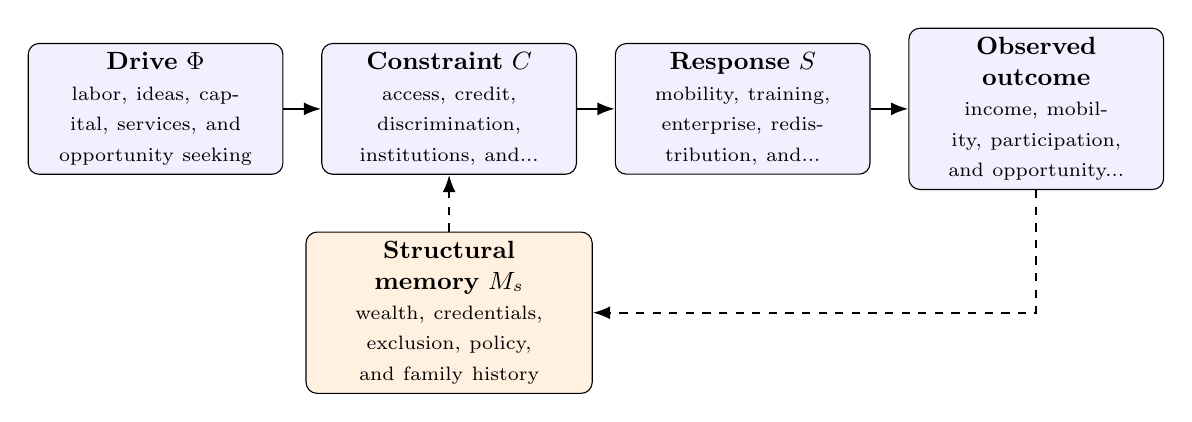
\begin{tikzpicture}[
    node distance=0.48cm,
    every node/.style={font=\small},
    box/.style={draw, rounded corners, align=center, minimum height=1.45cm, text width=3.0cm, fill=blue!6},
    memory/.style={draw, rounded corners, align=center, minimum height=1.25cm, text width=3.4cm, fill=orange!12},
    flow/.style={-{Latex[length=2.2mm]}, thick},
    feedback/.style={-{Latex[length=2.2mm]}, thick, dashed}
]
\node[box] (drive) {\textbf{Drive $\Phi$}\\\scriptsize labor, ideas, capital, services, and opportunity seeking};
\node[box, right=of drive] (constraint) {\textbf{Constraint $C$}\\\scriptsize access, credit, discrimination, institutions, and...};
\node[box, right=of constraint] (response) {\textbf{Response $S$}\\\scriptsize mobility, training, enterprise, redistribution, and...};
\node[box, right=of response] (outcome) {\textbf{Observed outcome}\\\scriptsize income, mobility, participation, and opportunity...};
\node[memory, below=0.72cm of constraint] (memory) {\textbf{Structural memory $M_s$}\\\scriptsize wealth, credentials, exclusion, policy, and family history};
\draw[flow] (drive) -- (constraint);
\draw[flow] (constraint) -- (response);
\draw[flow] (response) -- (outcome);
\draw[feedback] (outcome.south) |- (memory.east);
\draw[feedback] (memory.north) -- (constraint.south);
\end{tikzpicture}
\caption{Paper C-01 observable CDFD/AFL architecture for Economics and Opportunity. Solid arrows give the proposed forward chain; dashed arrows make history-dependent feedback explicit.}
\label{fig:c01-architecture}
\end{figure}

\subsection{Paper-Specific Causal Hypothesis}

For this paper, the hypothesized causal sequence is specific. A change in
labor, ideas, capital, services, and opportunity seeking arrives faster than mobility, training, enterprise, redistribution, and network support can compensate.
This raises or redistributes access, credit, discrimination, institutions, and geographic barriers. If the load persists,
the retained state encoded by wealth, credentials, exclusion, policy, and family history changes the next response, so a later event of equal
magnitude can produce a different trajectory in income, mobility, participation, and opportunity distribution. The
scientific task is to estimate that sequence against the best ordinary model of
the domain, not merely to redescribe the outcome after it occurs.

\subsection{Cross-Scale Translation Without Mechanistic Erasure}

For the socioeconomic systems family, the cross-domain translation compares human and institutional throughput, unequal access to capacity, adaptive coordination, and historical path dependence. The variables are not morally neutral: aggregation can hide who receives flow, who bears constraint, and whose prior losses become persistent memory. \cite{BarabasiAlbert1999,WattsStrogatz1998,Holling1973,Shannon1948}
The required scale declaration for this paper is months to generations; households to economies. At short
scales, the key question is whether the incoming drive is transmitted,
buffered, or diverted. At intermediate scales, response changes effective
capacity and network exposure. At long scales, retained structure can alter the
state space itself. A result is genuinely cross-scale only when the aggregation
rule is stated and the same conclusion is not an artifact of averaging.

\subsection{Evidence Ladder and Discriminating Tests}

\begin{table}[htbp]
\centering
\small
\caption{Evidence ladder for Paper C-01. Each rung can fail independently.}
\begin{tabularx}{\textwidth}{|p{0.17\textwidth}|X|X|}
\hline
\textbf{Test} & \textbf{Design} & \textbf{Discriminating result} \\
\hline
Proxy audit & Measure panel surveys, administrative records, labor flows, credit data, and network measures and preregister how each record maps to $\Phi$, $C$, $S$, $M_s$, and $Y$. & The mapping fails if proxies are non-identifiable, circular, or change meaning across cases. \\
\hline
Load ramp & Apply or observe an economic shock or policy change applied across unequal starting conditions while estimating the dominant constraint and response time. & A threshold claim requires a reproducible nonlinear change and uncertainty bounds, not a visually chosen breakpoint. \\
\hline
Recovery and memory & Match present load across units with different histories, then compare recovery paths. & The memory claim requires history-dependent divergence after current conditions are controlled. \\
\hline
Model comparison & Compare the baseline domain model with and without the CDFD/AFL state variables using held-out data. & The paper's stated falsifier is: history-sensitive constraints do not improve mobility or opportunity forecasts. \\
\hline
\end{tabularx}
\end{table}

\subsection{Research Programme and Boundary Conditions}

The immediate research programme has four steps. First, construct a documented
dataset from panel surveys, administrative records, labor flows, credit data, and network measures and retain raw units before normalization.
Second, fit a baseline domain model and report its calibration and out-of-sample
error. Third, add the smallest identifiable CDFD/AFL state extension and test
whether it improves prediction of income, mobility, participation, and opportunity distribution. Fourth, repeat the
analysis across the declared scale range and publish negative cases as part of
the cross-domain translation audit.

% END PART IV MAJOR CROSS-DOMAIN UPGRADE

\section{Conclusion}
Wealth inequality is a pathological defect in a thermodynamic transport network. By applying CDFD to macroeconomics, we model the hypothesis that hoarding capital via structural memory ($M_s$) and artificial constraints ($C$) is thermodynamically unsustainable. Ensuring robust, equitable economic opportunity is a practical requirement to maintain the $\Psi_s \approx 1$ equilibrium necessary for the long-term survival of the civilization.
\section*{Conflict of Interest} The author declares no conflict of interest.
\section*{Data Availability}
Part-specific runtime diagnostics are under each Part's \path{outputs/} directory.

Release-wide code: \path{Part_E_Synthesis/supplementary/}.

Generated summaries: \path{Part_E_Synthesis/outputs/}.

Figures: \path{Part_E_Synthesis/figures/}.


\section{Reference Layer}
\bibliographystyle{plain}
\bibliography{universal_afl_references}
\end{document}
